\documentclass[12pt,a4paper]{article}

\usepackage[T1]{fontenc}
\usepackage{amsmath, amssymb, amsfonts}
\usepackage[magyar]{babel}
\usepackage[utf8]{inputenc}
\usepackage{graphicx}
\usepackage{graphics}
\usepackage{mathtools}
\usepackage{epsfig}
\usepackage{epstopdf}
\usepackage{cite}
\usepackage{caption}
\usepackage{hyperref}
\usepackage[bottom=4cm]{geometry}
%\geometry{a4paper, portrait, margin=1in}

\title{\huge{Alkalmazott Fizikai Módszerek Laboratórium}\\ \vspace{20pt}
\textbf{Optikai pumpálás}}

\author{\Large{\textsc{Csörnyei Géza}} \vspace{10pt}\\
	\textrm{Eötvös Loránd Tudományegyetem}\\
	\textrm{Fizikus MSc I}
	}
\date{}
%\lhead{}
\begin{document}
\addtolength{\voffset}{-1.0cm}
\addtolength{\textheight}{1.0cm}
\begin{titlepage}
\maketitle

\begin{figure}[!htb]
\centering

\includegraphics[scale=0.6]{eltecimer.jpg}
\end{figure}

\hfil \Large{'E' mérőcsoport}\hfil  \\
\vspace*{2pt}
\hfil \Large{\emph{Mérés dátuma:} 2019.10.18.}\hfil \\
\vspace*{2pt}
\hfil \hspace*{45pt} \Large{\emph{Mérés vezetője:} Szabó Bálint}\hfil
\thispagestyle{empty}
\end{titlepage}

\section{Mérés célja}
\hspace*{10pt} Mérésünk célja, hogy a mérőhelyen található rubídium minta optikai pumpálását vizsgálva meghatározzuk a relaxációs időket, valamint a minta abszorpciós maximumaiból meghatározzuk a Föld mágneses terét és a mintában található izotópok g-faktorát.

\section{Elméleti összefoglaló}
 \hspace*{10pt} Az optikai pumpálás során a optikai besugárzás segítségével atomok, ionok energiaállapot szerinti eloszlását, például a Zeeman- vagy a hiperfinom felhasadás következtében megjelenő alnívók betöltését változtathatjuk meg. A mérés során három energianívóval dolgoztunk, melyet az alábbi sematikus ábra szemléltet:
\begin{figure}[!h]
\centering
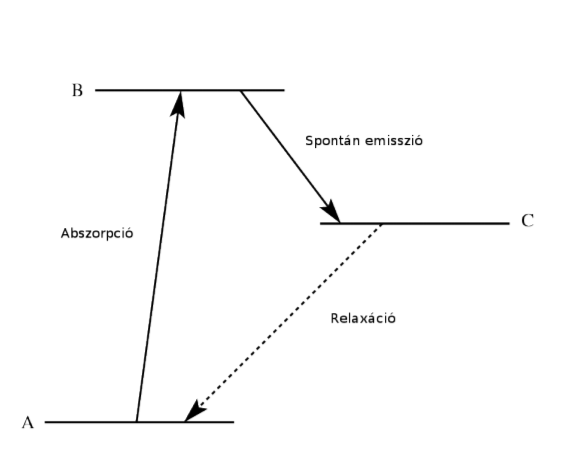
\includegraphics[scale=0.5]{nivok.png}
\caption{Optikai pumpálás három energianívó esetén}
\end{figure}
\newline
A megfelelő frekvenciával történő pumpálás esetén kialakulhat olyan helyzet, amikor a C állapot betöltöttség nagyobb lehet mint az A állapoté, de ez is csak egy bizonyos határig mehet el, ugyanis egy arány felett a folyamat telítődni fog. Az viszont nem fordulhat elő, hogy a B állapot betöltöttsége nagyobb legyen mint A-é, ez egy, az ábrán be nem jelölt folyamatnak, az indukált emissziónak köszönhető. A pumpálás során az abszorpció és az indukált emisszió folyamatok száma az alapállapoti illetve a gerjesztett atomok számától függ: mivel mind a két folyamathoz ugyanakkora energiájú foton szükséges, így amikor B betöltöttsége nagy lenne mint A-é, akkor az indukált emisszióból lenne több, tehát több gerjesztett atom esne vissza alapállapotba.\\
\hspace*{10pt} Az abszorpció, és így a szintek telítődésének mértékét a \cite{1} jegyzet szerint egy időállandóval vehetjük figyelembe. A szintek telítődése exponenciális felcsengést mutat ilyen karakterisztikus idővel. Ezen időállandó két részből tevődik össze: egyrészt a termikus relaxáció időállandójából, mely a hőmérsékleti egyensúly, azaz a kialakult mágneses momentumok (exponenciálisan lecsengő) bomlásának karakterisztikus ideje, másrészt a pumpálás karakterisztikus idejéből, mellyel az abszorpció során kialakult gerjesztett állapotok számát vehetjük figyelembe. Az összevont időállandó az alábbi képlettel adható meg:
\begin{equation}
\frac{1}{\tau}=\frac{1}{T_{p}}+\frac{1}{T_{1}}
\end{equation}
ahol $T_{P}$ a pumpálás, $T_1$ a termikus relaxáció időállandója.\\
\hspace*{10pt} Amennyiben a mágneses teret teljesen megszüntetjük, azaz a külső (Föld) mágneses térrel ellentétes irányú, de azonos nagyságú teret kapcsolunk, akkor a Zeeman-felhasadás eltűnik, csak két nívó marad, ekkor tehát pumpálni már nem lehet. Ez esetben a rendszer a termikus egyensúlyhoz relaxál, de ez gyorsabb mint a $T_1$ relaxáció, ezt, a külső mágneses térre merőleges irányú, azaz a transzverzális elektronspinek átfordulásához tartozó relaxációs időt $T_2$-vel jelöljük. Mágneses tér nélküli esetben ez a $T_1$-nél kisebb időállandó határozza meg a relaxációs folyamatot.\\
\hspace*{10pt} Ha az optikai pumpálás az alsó Zeeman-nívóról a felsőre történik, akkor a felső nagyobb energiával rendelkezik. A két nívó között az átmenet létrehozásának feltételét írja le a rezonancia-feltétel, mely 
$$h\nu = \mu_{B} g_{F} B_0$$
ahol $\nu$ a besugárzó elektromágneses tér frekvenciája, $\mu_{B}$ a Bohr-magneton, $g_{F}$ a g-faktor és $B_0$ a sztatikus feszítő tér, az alnívók kialakításához. A mérés során nem sztatikus teret használtunk, hanem egy sztatikus és egy szinuszos jel szuperpozícióját alakítottuk ki egy Helmholtz-tekercspár segítségével. Ennek lényege, hogy az rezonanciához szükséges mágneses teret periodikusan alakítjuk ki, így az oszcilloszkópon több abszorpciót is látunk majd periodikusan. Amikor az egyes abszorpciók egymástól időben azonos távolságra vannak, az esetben pontosan a rezonanciához szükséges mágneses teret állítottuk be. Ezen értéket feljegyezve, majd a polaritást megfordítva megmérjük ugyanígy a rezonanciához szükséges tér nagyságát, akkor más értéket fogunk kapni, a Föld mágneses tere miatt. Ezen két mérésből már meg tudjuk állapítani a Föld mágneses terének nagyságát, illetve a rezonanciához szükséges sztatikus tér nagyságát is, az alábbi módon:
$$B_{\textrm{Föld}}=\frac{B_0^{+}-B_0^{-}}{2} \hspace*{20pt} B_0=\frac{B_0^{+}+B_0^{-}}{2}$$
ahol a $B_0^{+}$ és a $B_0^{-}$ az egyes polaritások mellett mért mágneses indukciók értékeit jelölik.
\newpage
\section{Mérés menete}
\hspace*{10pt} A mérés első részében a relaxációs idők mérését végeztük el. A mérési összeállítás az alábbi volt:
\begin{figure}[!h]
\hspace*{-0.5cm}
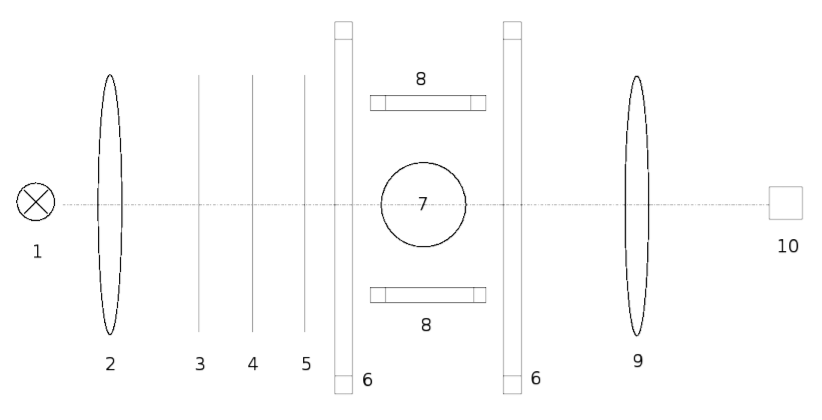
\includegraphics[scale=0.5]{osszeall.png}
\caption{A kísérleti berendezés vázlata. 1. Nagyfrekvenciás kisülési cső; 2. és 9. Gyűjtőlencse; 3. Interferenciszűrő; 4. és 5. Polarizációs szűrő és $\lambda/4$-es lemez cirkulárisan polarizált fény kialakításához; 6. Helmholtz-tekercspár; 7. Abszorpciós cső, melyben az optikai pumpálás történik; 8. Tekercspár rádiófrekvenciás tér létrehozására; 10. Fotodióda}
\end{figure}
\newline
A fotodiódát egy oszcilloszkópra kötöttük, melyet egy USB-kábellel a mérőhelyen lévő számítógépre csatlakoztattunk, mellyel elmentettük az oszcilloszkóp által mutatott képet. Két mérést végeztünk, az egyikben úgy állítottuk be a mágneses teret, hogy az átmenetek telítésbe menjenek, ezzel az összevont időállandót tudtuk mérni, másodszor olyan mágneses teret állítottunk be, hogy az az egyik polaritásnál pont ellentétes legyen a Föld mágneses terével, azaz az eredő tér nulla lett, így a $T_2$ relaxációs időt tudtuk megmérni.\\
\hspace*{10pt} A mérés következő részében a g-faktor meghatározásához szükséges mérést végeztük el. Négy különböző frekvenciájú mágneses tér esetén végeztük el az abszorpció vizsgálatát, azonban a frekvenciaértékeket nem tudtuk. Ennek meghatározására egy vezetőhurkot tettünk a mérőberendezésbe, melynek két végét az oszcilloszkópra kötöttünk, és így vizsgáltuk a kialakuló jelet, melyből a frekvenciát már meg tudtuk határozni.
\newpage
\hspace*{10pt} Az elméleti részben leírtakkal összhangban vizsgáltuk az abszorpciót a négy különböző frekvenciaérték esetén, mindkét polaritással. A mérés során csak a Helmotz-tekercsekre juttatott áramerősség értékét tudtuk feljegyezni, de mivel a Helmotz-tekercs jól meghatározott, közel homogén mágneses teret hoz létre egy adott áramerősség esetén, így a tekercs sugarának és menetszámának ismeretében egyértelműen meg tudtuk határozni a mágneses indukció értékeket.

\section{Kiértékelés}
\subsection{Relaxációs idők mérése}
\hspace*{10pt} A műszer bekapcsolása után négyszögjelet kapcsoltunk a mérőkörre; a négyszögjel váltakozó, abszolút értékben állandó, de periodikusan váltakozó előjelű mágneses teret keltett. Az előjelváltáskor a mintában a Zeeman-nívók helyet cserélnek, valamint az addig felépített polarizáció is elvész egy relaxációs folyamat során. Ennek a relaxációnak (exponenciális felfutásnak) az időállandóját (az összesített időállandót) egyszerűen a válaszjel illesztésével kaphatjuk meg. Az illesztéshez használt függvény alakja
\begin{equation}
f(x)=a\cdot \textrm{exp}(-b*(x-c))+d
\end{equation}
volt. A kapott jel és az illesztése látható a \ref{fig:illeszt1}. ábrán.\\
\begin{figure}[!h]
\centering
\hspace*{-0.5cm}
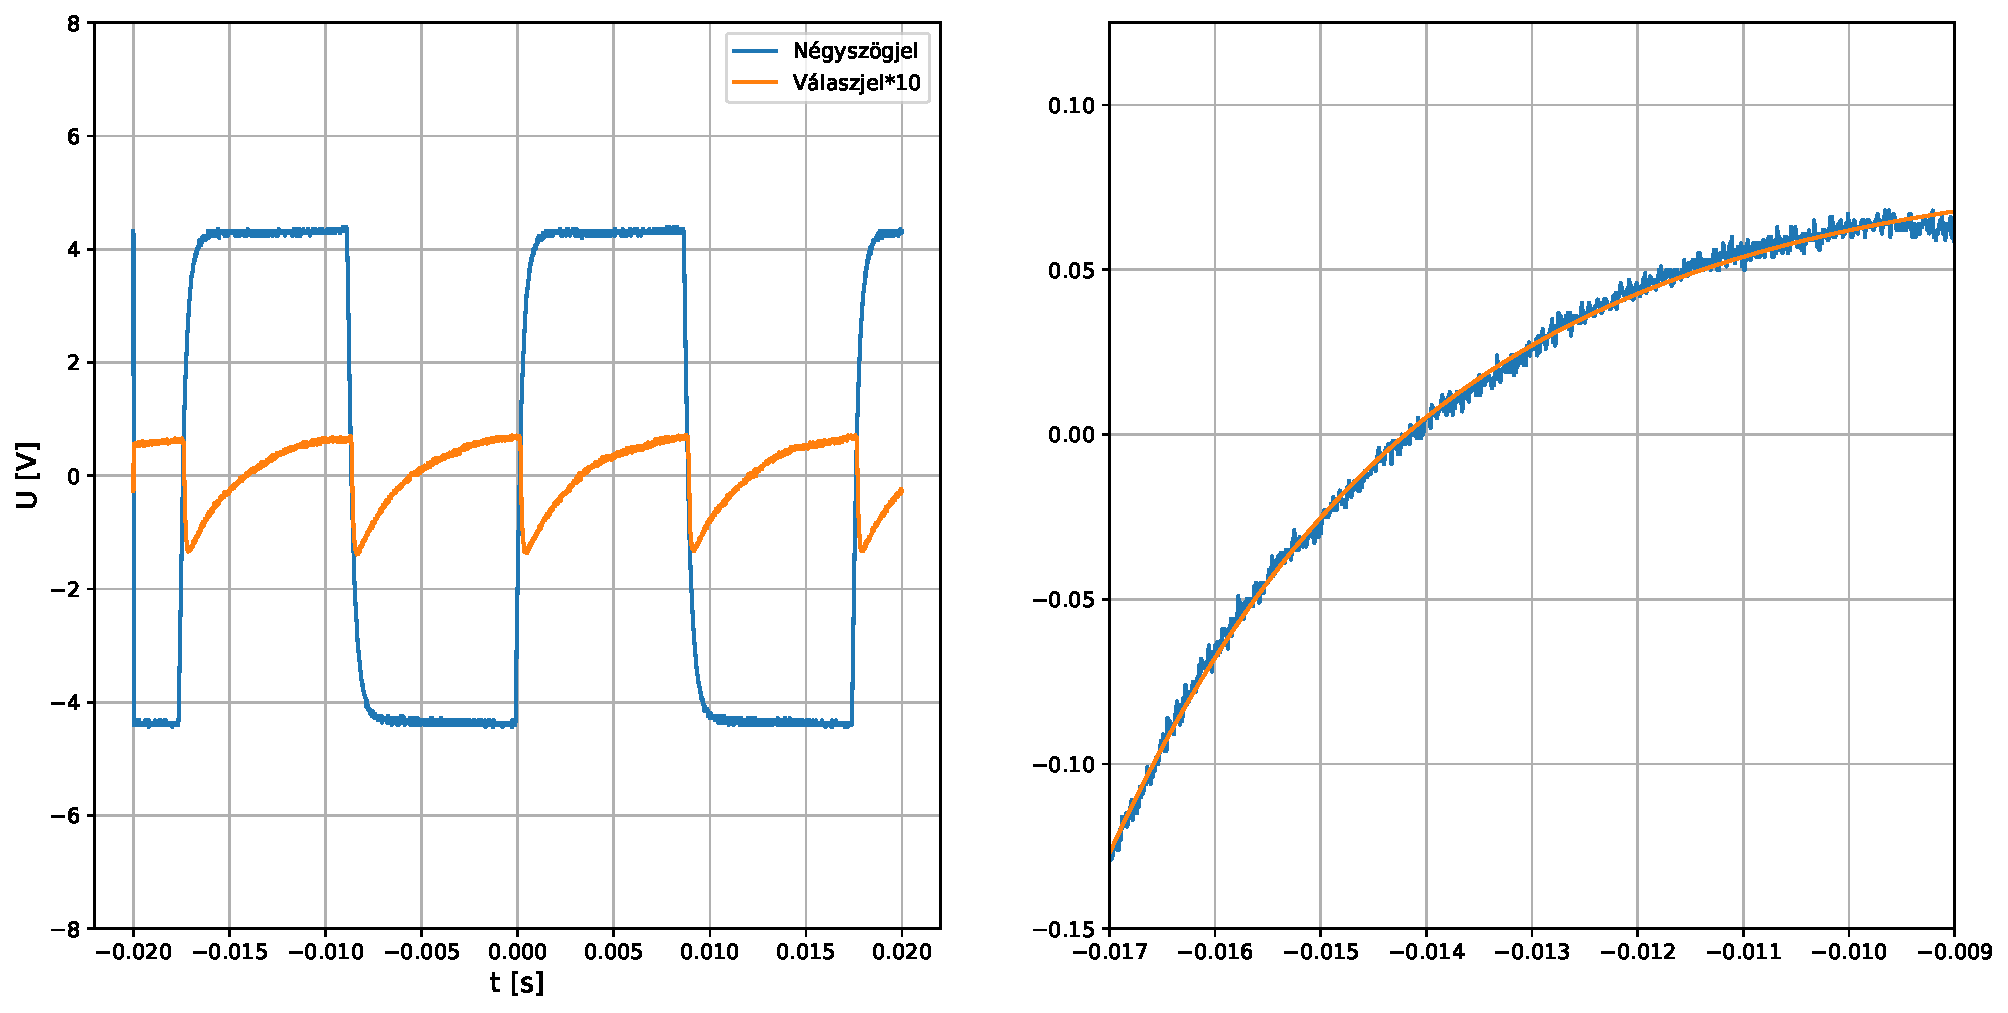
\includegraphics[scale=0.45]{tau_ill}
\caption{Az összesített időállandó meghatározása}
\label{fig:illeszt1}
\end{figure}
 \newline
 Négy egymás utáni relaxációs folyamatot rögzítettünk, ezek mindegyikét megillesztettem, majd a kapott időállandók átlagát vettem végleges értéknek. Az illesztésből kapott összesített időállandó értéke:
 $$\tau = (0.182 \pm 3.704\cdot 10^{-3}) \textrm{ ms} .$$
 Hasonló módon elvégeztem a Föld mágneses terének kioltása után felvett adatsort is, melyből a $T_2$ relaxációs időt tudtam meghatározni. A mért jel és az illesztés \ref{fig:illeszt2}. ábrán látható. \\
\begin{figure}[!h]
\centering
\hspace*{-0.5cm}
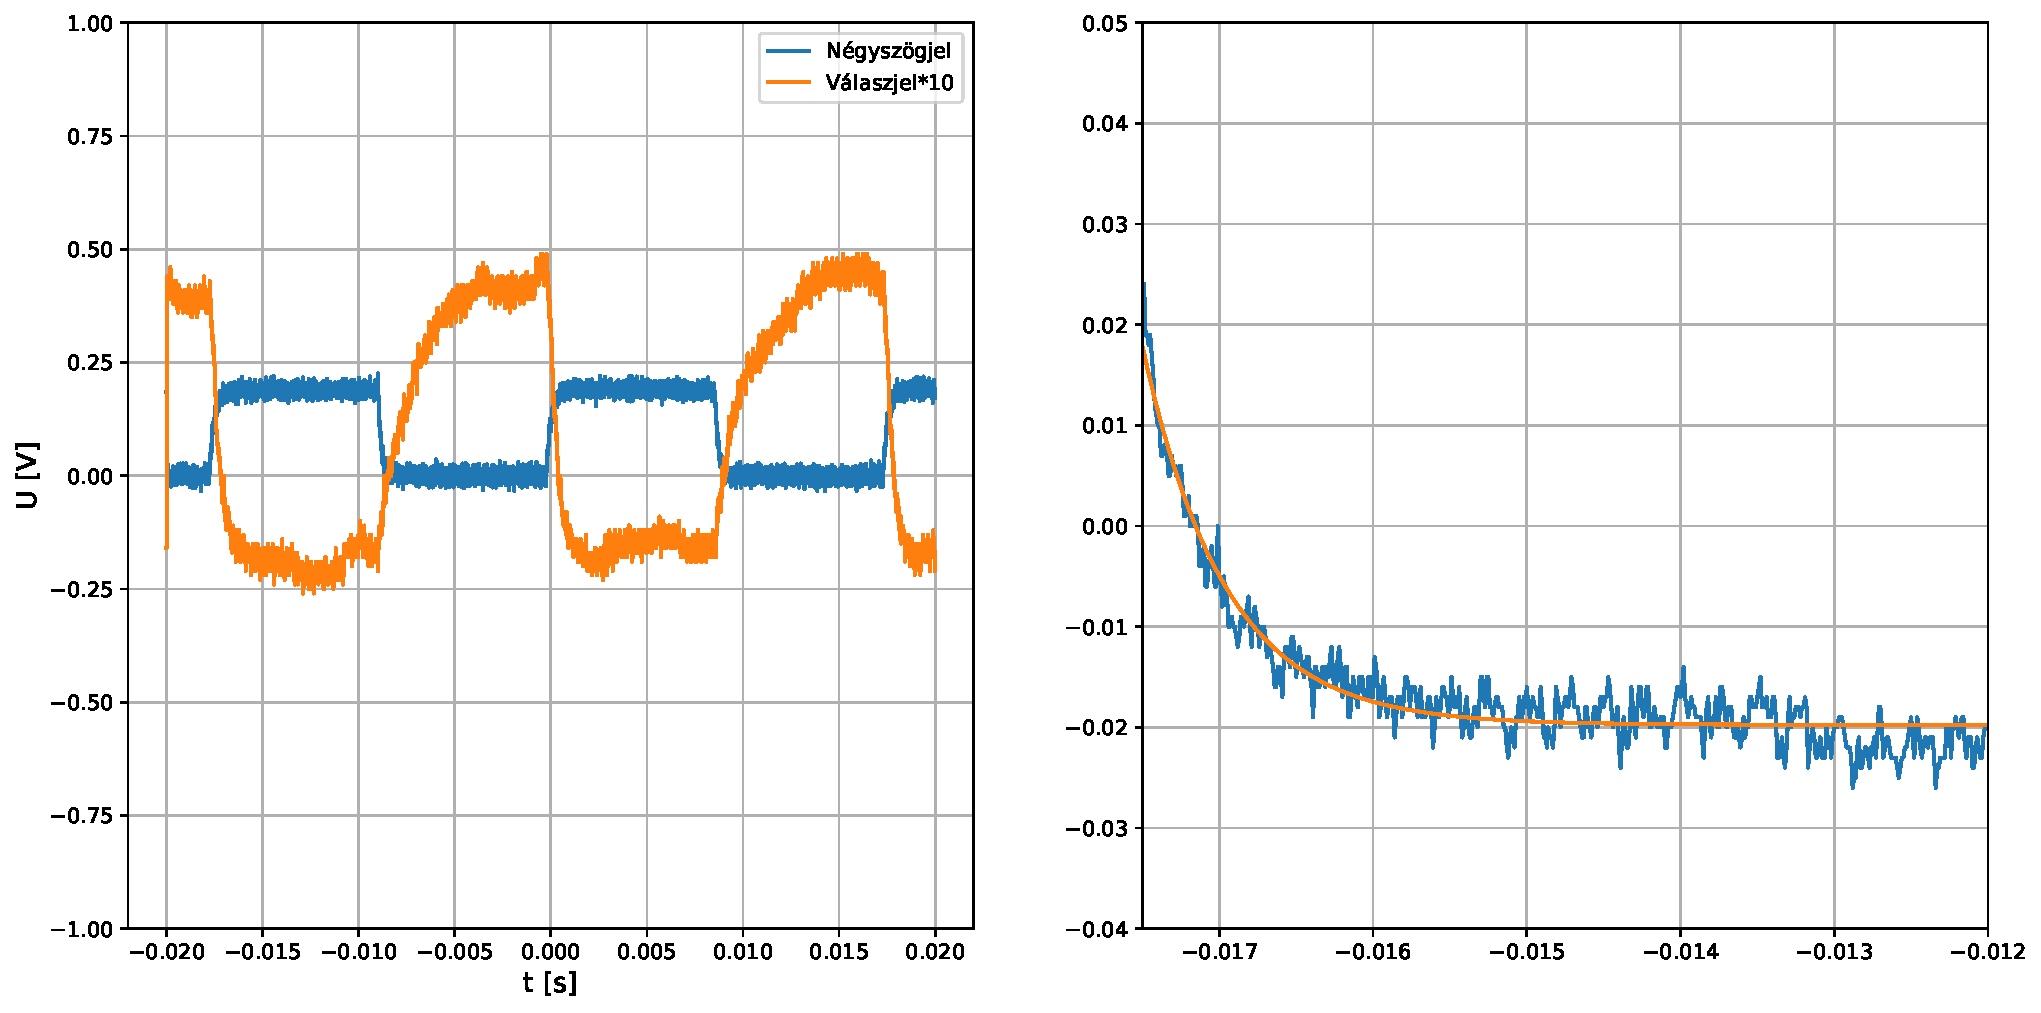
\includegraphics[scale=0.45]{t2_ill}
\caption{A $T_2$ időállandó meghatározása}
\label{fig:illeszt2}
\end{figure}
 \newline
 Az illesztésből kapott relaxációs idő:
 $$T_2 = (0.536 \pm 0.014) \textrm{ ms} . $$
\subsection{Rezonanciaátmenetek megfigyelése, g-faktorok meghatározása}
\hspace*{10pt} A rubídiumizotópok g-faktorainak meghatározásához végzett mérés során az egyes rezonanciákhoz tartozó Helmholtz-tekercsre kapcsolt áramot mértük meg. A mért értékek az alábbi táblázatban láthatók:
\begin{table}[!h]
\begin{center}
\begin{tabular}{|c||c|c||c|c||c|c||c|c|}
\hline
Frekvencia & \multicolumn{2}{|c||}{$\nu_4$} & \multicolumn{2}{|c||}{$\nu_6$} & \multicolumn{2}{|c||}{$\nu_7$} & \multicolumn{2}{|c|}{$\nu_8$}\\
\hline
Polaritás & + & - & + & - & + & - & + & - \\
\hline
$I_{1}$ [mA] & 164 & 130 & 195 & 160 & 284 & 250 & 212 & 179 \\
\hline
$I_{2}$ [mA] & 239 & 205 & 284 & 250 & 415 & 382 & 308 & 276 \\
\hline
\end{tabular}
\caption{Az egyes izotópok rezonanciáihoz tartozó áramerősség értékek. A + és - polaritás a Föld mérőberendezéssel párhuzamos terével egyirányú, illetve azzal ellentétes tereket jelöl. A mérés során az egyes gerjesztő elektromágneses tér frekvenciákat nem ismertük, így az egyes frekvenciaértékeket a mérőberendezésen látottak szerint indexeltem.}
\end{center}
\end{table}
\newline
Ezen áramerősségek a Helmholtz-tekercspár külső tagjára jutottak, a belső, szinuszos mágneses tér kialakításáért felelős tekercs bemenetén nem változtattunk. A további számolásokhoz ezen áramerősség értékeket át kellett számolni mágneses indukcióba, melyet Helmholtz-tekercsek esetén a következő képlet segítségével tehetünk meg \cite{2}:
\begin{equation}
B(R/2)=\left (\frac{8}{5\sqrt{5}} \right ) \frac{\mu_0 n I}{R},
\end{equation}
ahol $n$ a tekercs menetszáma (jelen esetben 80), $R$ pedig a sugara (a külső Helmholzt-tekercsé 19.3 cm volt). Mivel az így kialakított tér a Helmhotz-tekercsen belül jó közelítéssel homogén, ezért a tekercsen belül mért tér meg fog egyezni ezen értékkel minden pontban. Az így kiszámolt mágneses terek tehát:

\begin{table}[!h]
\begin{center}
\resizebox{\linewidth}{!}{%
\begin{tabular}{|c||c|c||c|c||c|c||c|c|}
\hline
Frekvencia & \multicolumn{2}{|c||}{$\nu_4$} & \multicolumn{2}{|c||}{$\nu_6$} & \multicolumn{2}{|c||}{$\nu_7$} & \multicolumn{2}{|c|}{$\nu_8$}\\
\hline
Polaritás & + & - & + & - & + & - & + & - \\
\hline
$B_{1}$ [mT]  & 0.1223 & 0.0969 & 0.1454 & 0.1193 & 0.2117 & 0.1864 & 0.1580 &  0.1334\\
\hline
$B_{2}$ [mT] & 0.1782 & 0.1528 & 0.2117& 0.1864 &  0.3094 & 0.2848 & 0.2296 & 0.2057 \\
\hline
\end{tabular}}
\caption{A számolt B értékek}
\end{center}
\end{table}

Mivel a kapott értékekre egyszer hozzáadódik, egyszer pedig levonódik a Föld mágneses tere, így az azonos frekvenciákhoz, de eltérő polaritásokhoz tartozó értékeket kiátlagolva kiejthetjük a Föld mágneses terének járulékát. Az így kapott értékek az alábbi táblázatban láthatók:
\begin{table}[!h]
\begin{center}
\begin{tabular}{| c || c || c || c || c ||}
\hline
Frekvencia & $\nu_4$ & $\nu_6$ & $\nu_7$ & $\nu_8$\\
\hline
$B_{1}$ [mT] & 0.1096 & 0.1324 & 0.1991 & 0.1457 \\
\hline
$B_{2}$ [mT] & 0.1655 & 0.1991 & 0.2971 & 0.2177 \\
\hline
\end{tabular}
\caption{Kiátlagolt B értékek}
\end{center}
\end{table}


Meg kellett továbbá állapítanom a $\nu_i$ frekvenciákat is, mivel ezek nem voltak adottak. Egy vezetőhurkot a mágneses térbe helyezve rögzítettük a jelet egy oszcilloszkóp segítségével (\ref{fig:frek}. ábra), majd a kapott adatsort Fourier analízis segítségével megillesztettem a periódusidő kinyeréséhez (\ref{fig:four}. ábra).\\

\newpage

\begin{figure}[!h]
\centering
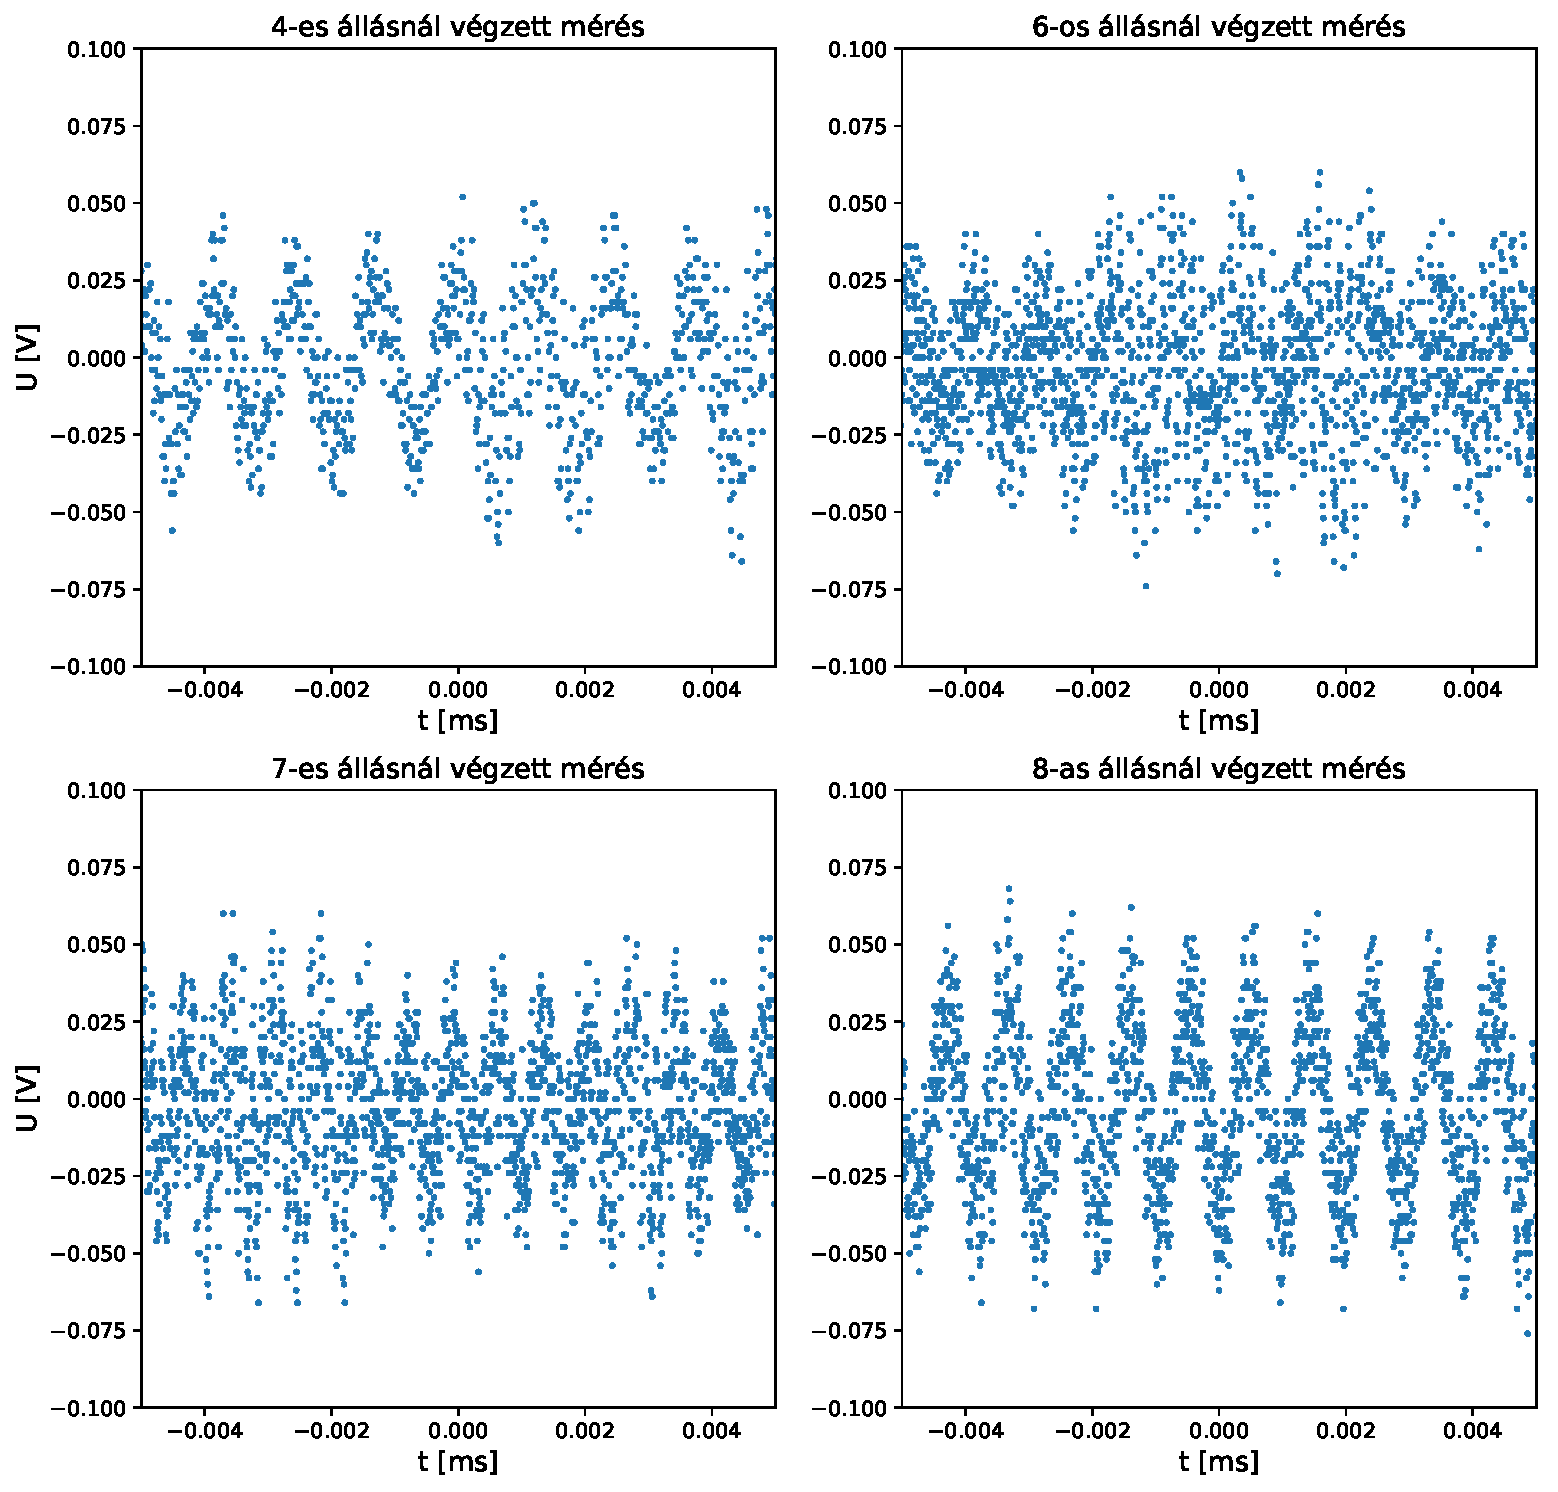
\includegraphics[scale=0.55]{frekik}
\caption{A vezetőhurok segítségével rögzített jelek}
\label{fig:frek}
\end{figure}

A Fourier analízis eredményeképp előálló frekvenciákat az alábbi táblázat tartalmazza:\\

\begin{table}[h!]
\begin{center}
\begin{tabular}{| c || c |}
\hline
Kapcsoló állása &  $\nu$ (Hz) \\ \hline
4 & $7.966\cdot 10^{5}$ \\ \hline
6 & $9.560\cdot 10^{5}$ \\ \hline
7 & $1.418\cdot 10^{6}$ \\ \hline
8 & $1.046\cdot 10^{6}$ \\ \hline
\end{tabular}
\caption{A frekvenciák}
\end{center}
\end{table}
\newpage

\begin{figure}[!h]
\hspace*{-1.0cm}
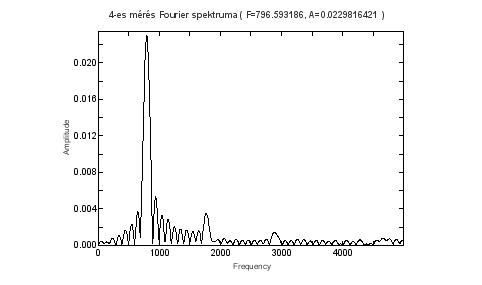
\includegraphics[scale=0.5]{4esFour}
\hspace*{-1.0cm}
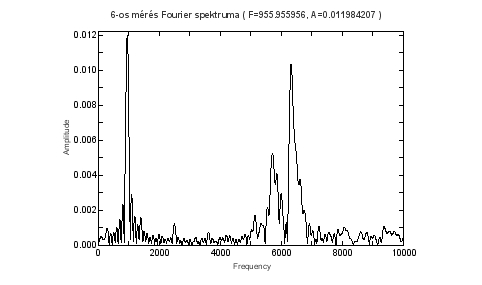
\includegraphics[scale=0.5]{6osFour}
\hspace*{-1.0cm}
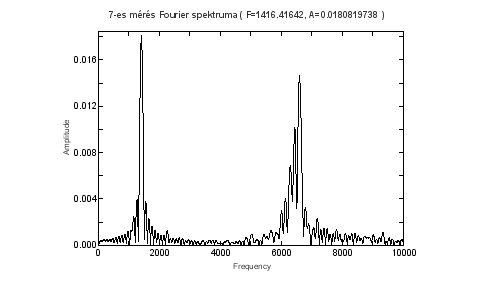
\includegraphics[scale=0.5]{7esFour}
\hspace*{-1.0cm}
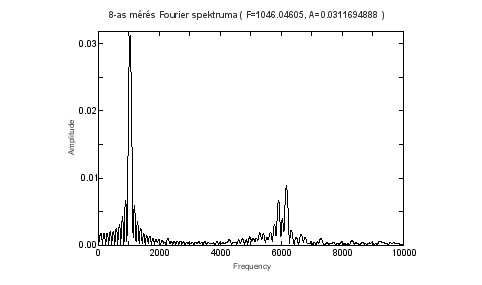
\includegraphics[scale=0.5]{8asFour}
\caption{Az egyes mérések Fourier spektrumai. A vízszintes tengelyen a frekvenciaértékek ms-ban értendők}
\label{fig:four}
\end{figure}



Ezután a g-faktorok meghatározásához a $h\nu-\mu_BB$ arányosságot kell vizsgálnunk a rezonanciafeltételnek megfelelően. Ennek értelmében a számolt adatokra egyenest illesztettem, melynek meredeksége megadta a keresett g-faktorok értékét.
\begin{table}[!h]
\begin{center}
\begin{tabular}{| c || c || c || c || c ||}
\hline
$h\nu$ [J] & $5.281\cdot 10^{-28}$ & $6.338\cdot 10^{-28}$ & $9.401\cdot 10^{-28}$ & $6.935\cdot 10^{-28}$ \\
\hline
$\mu_BB_{1}$ [J] & $1.016\cdot 10^{-27}$ & $1.226\cdot 10^{-27}$ & $ 1.846\cdot 10^{-27}$ & $1.351\cdot 10^{-27}$ \\
\hline
$\mu_BB_{2}$ [J] & $1.535\cdot 10^{-27}$ & $1.846\cdot 10^{-27}$ & $2.755\cdot 10^{-27}$ & $2.019\cdot 10^{-27}$ \\
\hline
\end{tabular}
\caption{A g-faktorok számolásához ábrázolandó mennyiségek}
\end{center}
\end{table}

\newpage

\begin{figure}[!h]
\centering
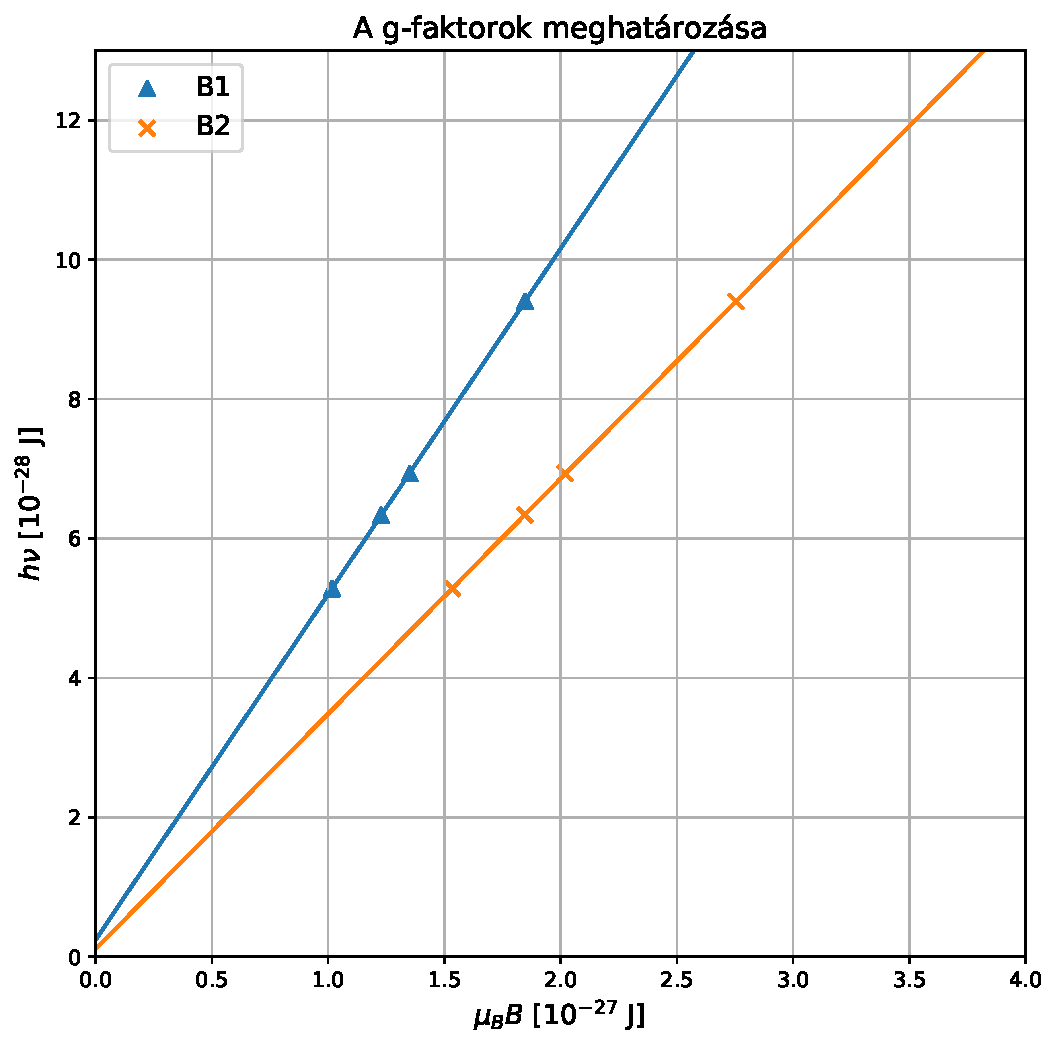
\includegraphics[scale=0.68]{g_faktor}
\caption{A kapott adatokra illesztett egyenesek}
\end{figure}


Az illesztett egyenesek egyenlete:
\begin{equation*}
\begin{split}
y_{B1}(x) = (4.9595\pm 0.0164)\cdot x +0.2428 \pm 0.0228,\\
y_{B2}(x) = (3.3736\pm 0.0120)\cdot x +0.1116\pm 0.0250.
\end{split}
\end{equation*}

Mivel már az illesztés során figyelembe vettük $h$ és $\mu_B$ mennyiségeket, így a g faktorok közvetlenül a meredekségből következnek (az illesztésnél használt eltérő nagyságrendek miatt a kapott egyenes meredekségek tizede lesz):
\begin{equation*}
\begin{split}
g_{F1} = 0.496,\enspace \delta g_{F1}=0.3\% \\
g_{F2} = 0.337,\enspace \delta g_{F2}=0.4\%
\end{split}
\end{equation*}

Mivel $g_{F1}\approx \frac{1}{2}$, ezért ez a 87-es tömegszámú Rb izotóphoz, valamint mivel $g_{F2}\approx \frac{1}{3}$, így ez a 85-es tömegszámú Rb izotóphoz tartozik.

\newpage
\subsection{Magspin meghatározása}
\hspace*{10pt} A méréshez használt \cite{3} függelékben található képlet alapján az egyes alnívók közötti energiakülönbség és a magspin kapcsolata az alábbi:
$$\Delta E=\mu_{B}B\frac{g_{J}}{2I+1}$$
ahol $I$ az általunk keresett magspin. Tehát az illesztésből kapott $g_{F}$ értékek és a $g_{J}$ értékek között az alábbi kapcsolat áll fenn:
$$g_{F}=\frac{g_{J}}{2I+1}.$$
Az egyes $g_{J}$ értékeket a Landé-formula alapján számolhatjuk, melyből azt kapjuk, hogy mind a két izotóp esetére $g_{J}=2$. Ez alapján tehát a keresett magspin a két izotóp esetére:
$$I_{85Rb}=\frac{1}{2} \left(\frac{g_{J}}{g_{F2}}-1\right)=2.464 \pm 0.009$$
$$I_{87Rb}=\frac{1}{2} \left(\frac{g_{J}}{g_{F1}}-1\right)=1.516 \pm 0.005$$
Ezen értékek közel megegyeznek a \cite{3} függelékben található értékekkel, melyek $I_{85Rb}=\frac{5}{2}$ és $I_{87Rb}=\frac{3}{2}$.

\subsection{A Föld mágneses tere}
A számolt B értékekből meg tudjuk állapítani a Föld mágneses indukciójának a mérési összeállítás-irányú vetületét is, ha nem átlagolunk, hanem a különbség felét képezzük:
\begin{equation*}
B_{\textrm{Föld}} = \frac{B_0^+ - B_0^-}{2}
\end{equation*}
\begin{table}[!h]
\begin{center}
\begin{tabular}{| c || c || c || c || c ||}
\hline
Frekvencia & $\nu_4$ & $\nu_6$ & $\nu_7$ & $\nu_8$\\
\hline
$B_{\textrm{Föld}_1}$ [mT] & 0.0127 & 0.0131 & 0.0127 & 0.0123 \\
\hline
$B_{\textrm{Föld}_2}$ [mT] & 0.0127 & 0.0127 & 0.0123 & 0.0120 \\
\hline
\end{tabular}
\caption{A számolt B értékek a Föld mágneses terére}
\end{center}
\end{table}

Az összes kapott értéket kiátlagolva megkapjuk a Föld mágneses terének mérési elrendezésre vetített nagyságát:
\begin{equation*}
B_{\textrm{Föld}} = 12.549\pm 1.301\enspace \mu T 
\end{equation*}
A Föld mágneses tere körülbelül $30-60\enspace \mu T$ nagyságrendbe esik,  ennek csak töredékét kaptuk mérésünk alapján, mely annak köszönhető, hogy a mérési elrendezés Kelet-Nyugati irányban állt.


\section{Diszkusszió}
\hspace*{10pt} Mérésünk során sikerült meghatároznunk a rubídiumizotópok g-faktorait, majd ezen értékekből az egyes izotópokhoz tartozó magspineket is, továbbá megmértük az optikai pumpálás folyamatához tartozó relaxációs folyamatok időállandóit és nem utolsó sorban meghatároztuk a Föld mágneses terének a mérés tengelyével megegyező irányú vetületét.


\begin{thebibliography}{99}

\bibitem{1} \emph{Kiadott jegyzet}:\\
\texttt{http://metal.elte.hu/oktatas/alkfizlab/meresleirasok/optpump.pdf}
\bibitem{2} \emph{A Helmholtz-tekercs terének levezetése}:\\
\texttt{https://www.didaktik.physik.uni-muenchen.de/elektronenbahnen/\\en/b-feld/B-Feld/Helmholtzspulenpaar.php}
\bibitem{3} \emph{A magspinek irodalmi értékei}:\\
\texttt{http://metal.elte.hu/oktatas/alkfizlab/meresleirasok/Afuggelek.pdf}

\end{thebibliography}

\end{document}
